\documentclass[palatino]{apuntesURJC}

\title{Educación, Sociedad y Familia}
\author{Víctor de Juan Sanz}
\date{16/17 C2}

% Paquetes adicionales
\newcommand{\profe}[0]{Ana Romero\xspace}

\begin{abstract}
Apuntes tomados en clase de la asignatura \textit{Educación, Sociedad y Familia}, impartida por \profe, doctora en Filosofía y profesora en la URJC.
\end{abstract}
% --------------------

\begin{document}
\pagestyle{plain}
\maketitle

\tableofcontents
\newpage
% Contenido.


\chapter{Educación}

\section{Ideas previas}

El \concept[Saber\IS práctico]{saber práctico} es el que se aprende en el hacer.
%
Que se aprenda haciendo no significa que no haya teoría.
%
Por ejemplo, la educación es un saber práctico.


El \concept[Saber\IS pragmático]{saber pragmático}, sólo si sirven para algo.
%
Reducir el saber práctico al saber pragmático, nos cargamos la esencia.
%
Con las personas por ejemplo, se ve claro.
%
Una persona se valora por lo que es, no para lo que sirve.


La educación se puede considerar un arte.
%
No es una mera aplicación técnica ni de recetas.

La reflexión no es un lujo sino un elemento indispensable.
%
Para guiar esta reflexión, hay 4 preguntas fundamentales, que hacerse en orden:
%
\begin{itemize}
	\item ¿Qué? ¿Qué estoy haciendo? ¿Qué están aprendiendo?
	\item ¿Porqué? ¿Porqué quiero hacer esto? ¿Porqué un alumno no se comporta bien?
	\item ¿Para qué? ¿Para qué quiero hacer esto? ¿Para qué
	\item ¿Cómo? \subitem Solamente cuando las 3 anteriores están contestadas, tiene sentido preguntarnos por el cómo.
\end{itemize}



\textbf{Conclusión}

Hay que hacer para aprender, pensando sobre el sentido de la acción educativa (la teoría: el porqué y el para qué de lo que hago) y pensando también sobre la propia acción para mejorarla.

\subsection{La Educación como fenómeno humano}

El hombre es el único animal que necesita aprender a comportarse como lo que es, como ser humano.
%
Además, puede comportarse como lo que no es, puede comportarse inhumanamente.

El ser humano necesita de otros seres humanos para aprender.
%
Los casos de seres humanos salvajes (criados en la naturaleza), con inmensas dificultades para socializar, avalan este argumento.
%
El resto de animales tienen una \textbf{dotación instintiva} mucho mayor.
%
Si a un animal lo abandonas con animales de otra especie, desarrolla comportamientos de la especie, debido a los instintos.
%
En el ser humano, no ocurre tal.

El ser humano tiene 3 aspectos que hacen que el ser humano pueda ser educado.
\begin{itemize}
	\item \textbf{\concept[Indeterminación\IS Biológica]{Indeterminación biológica:}} el ser humano nace inacabado, tanto a nivel cultural como a nivel fisiológico.
	%
	Esto permite (y a la vez exige) el aprendizaje.
	\subitem Es clave en este aspecto la racionalidad del hombre.
	\item \textbf{Libertad:} tomar las propias decisiones y de elegir los propios fines a los que uno se dirige y a los que dirige su vida.
	\item \textbf{Trascendencia (capacidad) y necesidad del otro:} El ser humano es un animal social.
\end{itemize}

Vamos a seguir profundizando.

Delval, un psicólogo español de gran renombre, acuñó el término \concept[Plasticidad]{plasticidad}.
%
La capacidad de seguir aprendiendo. Además, esta capacidad es muy grande.
%
No hay fin para el aprendizaje del hombre, tampoco a nivel neurobiológico, como constatan los últimos estudios.

La plasticidad humana se muestra también en la mano.
%
La mano no tiene una funcionalidad concreta, como son las membranas de un palmípedo \footnote{rana}.
%
Al no tener una funcionalidad concreta, decimos que es abierta, que tiene una \concept[Indeterminación\IS funcional]{indeterminación funcional}.


Ortega dice:

La educación es una necesidad natural y es de carácter cultural.
%
Es natural por lo constatado anteriormente.
%
Y decimos que su carácter es cultural, porque la manera de educar depende de la cultura.
%
Se educa distinto en las distintas culturas y en las distintas épocas.


Existen 4 aptitudes que sitúan al hombre en diferente plano al resto de vivientes.
\begin{itemize}
	\item \textbf{Utilización de un \concept[Lenguaje\IS simbólico]{lenguaje simbólico}} El ser humano utiliza un lenguaje de signos para transmitir el pensamiento y para comunicarse. El lenguajes simbólico es exclusivo del ser humano.

	Otros lenguajes que utilizan ciertas especies animales (las más desarrolladas) es el \concept[Lenguaje\IS Dígito]{lenguaje dígito}.
	%
	Este lenguaje está siempre asociado a expresar sus necesidades o las necesidades de su especie.
	%
	El lenguaje simbólico va más allá de simplemente expresar necesidades. Por ejemplo, la poesía.

	\item \textbf{El uso de la técnica} La utilización de la naturaleza para crear herramientas.
	\item \textbf{La ética} la distinción entre el \textit{ser} y el \textit{deber ser}.
	\item \textbf{El arte} La producción de objetos artísticos solamente es propia del ser humano.
\end{itemize}

Como el ser humano es educable, es también manipulable. Precisamente porque tiene tanto por aprender, precisamente por la plasticidad, puede ser manipulado.
%
Cuando hablamos de \concept[Manipulación]{manipulación} hablamos de un uso abusivo del carácter conductor del proceso educativo que no deja lugar o que ahoga la libertad personal y que niega o ahoga el enfrentamiento del educando con la realidad que vive.
%
¿Qué ocurre en las actitudes manipulativas? Muestran que se trata a la persona como un medio al servicio de los propios fines.
%
Además, se silencian algunas de las dimensiones de la libertad.

¿Cómo evitar la manipulación?
%
Para evitar la manipulación, hay que buscar el bien del educando.
%
Lo que diferencia la acción manipulativa de la acción educativa es el fin.
%
La manipulativa es según los  fines del manipulador, la educativa es según los fines particulares del educando.

Lo más esencial para evitar la manipulación es hacerles capaces de pensar por sí mismos.
%
Y no sólo hacerles capaces de pensar por sí mismos, sino de que tengan ese \textbf{hábito}.

Otra posibilidad es mostrar el fin que se busca con la acción educativa.


\textit{En la educación formal:}
Para evitar la manipulación en la actitud educativa es bueno incluir y hacer partícipes a los padres.
%
Esta acción evita la manipulación por parte del profesor. ¿Por qué?
%
Lo habitual es que los padres busquen el bien de sus hijos. Así, el contar con las padres en la acción educativa, ejerce como pared de contención.


\section{La persona y la educación}

Vamos a ver 5 notas que describen a la persona. Estas 5 notas se llaman \concept[Aspecto Fenomenológico]{aspecto fenomenológicos}.

\begin{itemize}
	\item \textbf{Intimidad:} Todos los seres vivos tienen como característica \textit{inmanecia}.
	%
	Lo que se guarda y lo que queda dentro.
	%
	Todo ser vivo lleva a cabo acciones inmanentes, todo ser vivo tiene un mundo interior.
	%
	El ser humano en concreto, tiene un mundo interior que solamente cada ser conoce (salvo que decida darlo a conocer).
	%
	Ese mundo interior que existe en las personas, es un mundo en el que cada uno se puede introducir; cada uno puede adentrarse, sumergirse en su propia intimidad.
	%
	Además, ese adentrarse/sumergirse puede hacerse sin que nadie se de cuenta.
	%
	Por otro lado, es un mundo al que puedo abrirme: ¿Cuáles son mis deseos? ¿Cuáles son mis criterios?
	%
	En lo que llamamos adolescencia del ser humano, se produce el descubrimiento del mundo interior. \footnote{Este es uno de los grandes descubrimientos de la adolescencia.}

	\subitem Esta intimidad puede crecer y hacerse más profunda.

	\subitem Lo íntimo es tan esencial que tiene un sentimiento propio que la protege: la vergüenza.
	%
	Cuando nuestra intimidad aparece al descubierto, aparece \textit{naturalmente} el sentimiento de vergüenza o pudor.

	\item \textbf{Manifestación:} La capacidad para sacar de sí mismo la intimidad.
	%
	La manifestación de la intimidad se hace a través de 3 vías:
	\subitem \textbf{Cuerpo: } Es un mediador entre la interioridad y la exterioridad. La persona manifiesta su intimidad a través del cuerpo.
	%
	Lo que llamamos \concept[Lenguaje\IS no verbal]{Lenguaje no verbal}
	%
	Esto se ve especialmente en una parte del cuerpo: el rostro.
	%
	Incluso, dentro del rostro, la mirada es especialmente expresiva.\footnote{Por ejemplo, cuando quieres ignorar a alguien, dejas de mirarle.}


	\subitem \textbf{Lenguaje:} \footnote{entendiendo lenguaje como lenguaje verbal.}
	%
	A través del lenguaje hago público, comparto con otros aquello que antes estaba dentro de mi.

	El lenguaje tiene mayor capacidad expresiva que el cuerpo y puede permanecer (a través de la escritura sobretodo).

	\subitem \textbf{Acción:}
	%
	Las personas nos damos a conocer con nuestros actos.
	%
	La persona no es sólo sus acciones, pero es aquello que hace. \footnote{No sé si esta afirmación es lógicamente consistente en sí misma.}

	\item \textbf{Libertad:} el ser humano es dueño de sí mismo.
	%
	Es principio y origen de sus actos. Ahora bien, al ser dueña de sus actos, es también dueña de su vida y de su destino.

	\subitem El hombre es esencialmente libre. Aunque tenga mermadas sus libertades (como podría ser una persona en un campo de concentración), la libertad sigue siendo posible.
	%
	Siguen existiendo decisiones que tomar, entre ellas:

	\item \textbf{Capacidad de dar-darse-autoposeerse-libertad: autotrascendencia}
	Llamamos \textit{darse} cuando una persona extrae algo de su intimidad y se lo da a otra persona que lo acepta.

	El ser humano puede dar:

	\subitem \textbf{De lo que hace}

	\subitem \textbf{De lo que tiene:} antropológicamente más complejo. Hay 2 niveles del tener: el nivel material y el nivel inmaterial.
	%
	El hombre puede prestar sus posesiones (un coche) y puede prestar consejo, su experiencia...

	\subitem \textbf{De lo que es:} Este es el nivel más profundo de donación.
	%
	Esa capacidad de dar y de recibir lo dado, se llama \concept[Amor]{amor}.
	%
	Y la intimidad personal se nutre, entre otras cosas, de lo que otros dan.

	\item \textbf{Carácter Dialógico:} El ser humano es el ser que habla.
	%
	El hombre es constitutivamente dialogante, ya que el hombre necesita hablar (hablar, no sólo comunicarse
	%
	\footnote{Porque la verdadera comunicación humana, en todo su espectro, no puede darse de manera completa sin el lenguaje, y además el lenguaje oral, que es la manera más rica de comunicarse.
	%
	Las personas que están privadas del lenguaje oral, ven mermada su capacidad de abstracción})
	%
	para desarrollarse.

\end{itemize}

%% Segunda clase.

\subsection{Dimensiones de la persona}

El ser humano es un ser complejo. 
%
Esto no significa psicológicamente complicado, sino que es un ser complejo.
%
Esta complejidad se puede observar en las diversas dimensiones de la persona.
%
El hombre tiene una dimensión \textbf{física}: tenemos un cuerpo físico, podemos tocar otras personas, etc. Además, hay una dimensión \textbf{afectiva}.  
%
El ser humano tiene sentimientos y emociones.
%
Desde el punto de vista de la psicología, se habla de las emociones como una respuesta tridimensional:  fisiológica, cognitiva y conductual.
%
\footnote{Para que aparezca un sentimiento tiene que haber un estímulo desencadenante.
%
Si el sentimiento que aparece es el miedo, puede darse sudoración, dolor de tripa... Esto son respuestas fisiológicas.
%
Además de la respuesta fisiológica, el sentimiento ofrece información: la relación entre la realidad (examen) y yo mismo. [Respuesta cognitiva].
%
Por último, hay una conducta expresada: no presentarse al examen (por ejemplo).
%
Esto sería la dimensión conductial.}
%
Por otro lado, hay una dimensión \textbf{psíquica}, tiene voluntad y puede tomar decisiones.
%
La dimensión psíquica incluye 2 facultades: inteligencia y la voluntad, cuyas operaciones son: conocer y querer respectivamente.
%
Pero el ser humano no es sólo esto.
%
Tiene una dimensión social: tiene capacidad y necesidad del otro.

Por último, como bien distingue \textit{Víctor Franquel} existe una \concept[Dimensión\IS de sentido]{dimensión de sentido}, también llamada existencial o personal.
%
La búsqueda del sentido: ¿ser o no ser? Como decía Sarte: ¿Porqué el ser y no la nada?
%
El sentido de la existencia se describe en esta dimensión (de ahí el nombre de la dimensión).

Un aspecto importante es que estas dimensiones están imbricadas. 
%
No son partes inconexas, sino que forman parte de una misma unidad que es la persona. 

Veámoslo con un ejemplo: estamos ante una puesta de sol. 
%
El sentido de la vista, nos permite una percepción puramente física que es la gama de colores que estamos viendo.
%
Además, pueden aparecer sentimientos: nostalgia por la vida rural, grandeza, agradecimiento, etc
%
Pueden despertarse voluntades: "Quiero hacer una foto" y pueden despertarse preguntas: "¿Porqué sale el sol?, ¿Porqué se forman estos colores?".
%
Puede ser que quiera disfrutarla con otra persona (dimensión social). 
%
Pero hay muchos más ejemplos. 
%
La somatización de las preocupaciones sería otro caso.

Esta conexión entre las dimensiones hace que no podamos acercarnos al hombre sólo desde una perspectiva, ya que daría lugar a errores.
%
Por ejemplo, las figuras tridimensionales vistas desde una perspectiva, pueden parecer iguales (la proyección sobre el plano horizontal de un cono, un cilindro y una esfera son iguales. Tienen la misma proyección, pero son figuras distintas).
%
Algo parecido ocurre con las personas.
%
Hay varias dimensiones y no podemos sólo fijarnos en una. 
%
Bien es verdad, que dependiendo de la edad vital de un ser humano, hay dimensiones más prominentes que otras.
%
El desarrollo de la dimensión física de la infancia es más importante.
%
A pesar de que el desarrollo físico sea más prominente es importante que \textbf{las  dimensiones crezcan armónicamente}.

La educación tiene que intentar armonizar estas dimensiones.
%
Y esta armonización en el hombre sólo se consigue si las dimensiones crecen (Polo).
%
El desequilibrio no se arregla capando las dimensiones que han crecido de más (normalmente), sino que hay que buscar que crezcan las dimensiones más atrasadas.

\paragraph{Educar personas es educar para la vida}
Educar es educar para saber vivir. 
%
Es mucho más amplio que instruir o que capacitar la inteligencia.
%
Un educador tiene que ser capaz de mirar hacia el futuro, tiene que saber ver el potencial de cada persona.



Tiene que atenderse el saber coger las riendas de la propia vida.


Pero, ¿qué significa saber vivir? Podemos desglosarlo en 3 aspectos: saber, saber hacer y saber ser.
%


\subsection{Agentes de la educación}

El agente principal de la educación es el propio educando, cuya función vital no es enseñar sino aprender.


Además, hay otros agentes secundarios, que además son agentes externos.
%
Los agentes externos más importantes son la familia, las instituciones educativas y la sociedad
%
\footnote{Por ejemplo, la sociedad occidental transmite valores como la democracia que en sociedades tribales no se transmiten}.

En España, las instituciones educativas tienen una incidencia temporal clarísima. 
%
La cantidad de años que una persona española participa en una institución educativa es muy longevo.


Este aprendizaje constituye la actividad principal del proceso. 
%
La labor del educador es de asistente. 
%
El educador tiene que ayudar a crecer al educando, pero si el educando no quiere aprender, no sirve de nada el educador.
%
Por esto, y ya lo decían los griegos, se considera que la profesión es una profesión asistencial.

Las potencialidades, las capacidades de la persona no se actualizan solas, por eso es necesaria la participación del educador en el proceso. 

\subsection{La acción educativa}
Anteriormente decíamos que educar es un saber que consiste en un "saber hacer". 
%
Es por ello que es necesario reflexionar sobre el \textit{hacer}.


Por ello, al estudiar la acción educativa es necesario estudiar el fin de la acción educativa, porque sino es difícil entender la educación.

Vamos a estudiar el fin de la educación según el modelo clásico (de Stanford).

El fin de la educación es el crecimiento humano en todas sus dimensiones especialmente de las potencias propiamente humanas, que son las potencias racionales.
%
Este planteamiento se queda un poco cojo, ya que la dimensión afectiva por ejemplo, no está tomada muy en cuenta.

\paragraph{La acción educativa es compleja:} implica enseñar y aprender. 
%
Estas 2 acciones son ontológicamente diferentes.

Pequeño anexo filosófico: existen acciones praxis (inmanentes) y acciones poiesis (transeunte). 
%
Una \concept[Acción\IS inmanente]{acción inmanente} cuyo resultado queda dentro del sujeto que la realiza. No queda modificado nada externo al sujeto, sino que lo que realmente queda modificado es el sujeto.
%
Sin embargo, la \concept[Acción\IS transeúnte]{acción transeúnte} es una acción cuyo resultado queda fuera del sujeto que la realiza.
Por ejemplo, aprender es una acción inmanente y construir es una acción transeúnte.

Aunque no sea muy relevante, esta distinción en algunos casos no está muy claro. 
%
Puede ser que la construcción de un edificio haya tenido efectos dentro del sujeto que las realiza.

Esta diferenciación es útil porque, predominantemente, enseñar es una acción transeúnte, mientras que aprender es una acción inmanente.
%
Al ser el aprendizaje una acción inmanente, ocurre que no hay resultados visibles de cómo ha ocurrido esa acción.

La enseñanza se subordina al aprendizaje.
%
Hay verdadera enseñanza cuando se suscita el aprendizaje del alumno.

\subsubsection{Acción de aprender} 

Desde la pedagogía, se considera que la \concept{formación} es un crecimiento o perfeccionamiento del alumno.
%
Como hemos dicho, el enfoque clásico se centra sobretodo en las potencias racionales, y es por ello que vamos a centrarnos en ellas nosotros también.


\subsubsection{Una propuesta: ayudar a crecer}

La educación es una acción del orden del obrar. 
%
Esta acción es intencional ya que busca un fin, ayudar al perfeccionamiento humano; entendiendo perfeccionamiento de una manera integral: se refiere al hombre entero, a todas sus dimensiones.

Además, la acción es recíproca (suscita acción del otro) y una reciprocidad de ayuda: la actualización de las potencialidades humanas no se da de modo autónomo.

El perfeccionamiento humano se ordena \textit{a y desde} la razón, sin excluir otras facultades humanas. 
%
Y las potencias racionales crecen a través de los hábitos.
%
Por ello, la acción educativa no puede limitarse a transmitir conocimientos ni a producir habilidades técnicas, sino que debe suscitar el crecimiento de los hábitos de la inteligencia y la voluntad.
%
Es esto lo que permite que crezca la propia potencia del educando.
%
El educando se está haciendo a así mismo más capaz mediante el desarrollo de ámbitos.

Por otro lado, el crecimiento no se identifica con el obrar, porque el hombre siempre es capaz de seguir creciendo aunque sus obras no cambiaran. 
%
La capacidad de crecer del hombre es irrestricta.\label{Capacidad_irrestricta}
%
John Dewey es un tipo que desde los años 50 del año pasado ha tenido mucha influencia con sus estudios.
%
Uno de ellos trata sobre un caso real: un grupo de universitarios había ganado un concurso de educación cívica y como celebración, destrozaron algunas aulas de la universidad.
% 
El comportamiento demostrado no es nada cívico, aunque al parecer, su conocimiento era excelente.
%
De casos como este concluimos que el conocimiento no se identifica con el obrar y que es necesario educar en hábitos y no sólo en conocimiento.
%
Esto es importante porque a veces nos centramos demasiado en los resultados.
%
El crecimiento tiene que manifestarse en las obras, pero no es lo único que valorar. Esa manifestación en obras, puede ser incompleta o insuficiente.


Aristóteles distingue hábitos teóricos de prácticos.

Los \concept[Hábitos\IS teóricos]{hábitos teóricos}  son los que se refieren a la inteligencia. Se refieren a  desarrollar la capacidad de elaborar conceptos, juicios y de razonar. 

Por otro lado, los \concept[Hábitos\IS prácticos]{hábitos prácticos} son los hábitos de la voluntad.
%
Algunos hábitos de la voluntad son: solidaridad, constancia, orden... 
%
Estos hábitos se adquieren por repetición de acciones y se agrupan en 4: moderación o templanza, coraje o fortaleza, justicia y prudencia.





\chapter{Condiciones, elementos y ámbitos para Educar}

\section{Condiciones necesarias}

El maestro no causa el crecimiento del alumno. Quien crece es el educando, el educador solamente pone condiciones para que se de ese crecimiento.

Vamos a ver cuáles son las condiciones necesarias para que se de un buen proceso de educación.




	\subsection{Aceptación}

	"Si comprendes, las cosas son como son. Si no comprendes, las cosas son como son" (Proverbio hindú)

	La realidad es tozuda y \textbf{no es lo mismo aceptar que comprender}. 
	%
	El hombre no comprende absolutamente todo lo que pasa a su alrededor, pero es necesario aceptar que la realidad es como es, la comprendamos o no.
	% 
	Y la aceptación de la realidad se da en varios aspectos que necesitan ser educados.

	\begin{itemize}
		\item \textbf{Aceptarse a uno mismo:} Esta dimensión tiene que ver con el realismo. 
		%
		Nace de saberse esencialmente valioso por ser, no por cómo se es ni por lo que se es.
		%
		Además, es necesario asumir con realismo con aceptación las posibilidades y límites.

		\item \textbf{Aceptar a los demás:} querer como son y no como queremos que sean.

		\item \textbf{Aceptar las circunstancias:} No podemos elegir las cartas que nos tocan, pero podemos elegir cómo jugarlas.
	\end{itemize}

	El primer paso para poder enseñar la aceptación es \textit{aceptar a los educandos como son}.
	%
	Si nosotros no les aceptamos, difícilmente podrán aprender a aceptarse y les costará aceptar a otros.
	%
	Además, es labor del educador ayudar al educando a conocerse: hacer ver con realismo las posibilidades y límites del educando. 

	Por último es importante distinguir aceptación de resignación. El hombre es libre y es el principio de sus actos.
	Por otro lado, el hombre es capaz de crecer y por tanto de cambiar, siendo esta capacidad irrestricta, como ya dijimos en \ref{Capacidad_irrestricta}.
	


	\subsection{Aprecio}

Es muy importante que los educadores seamos conscientes de la importancia del vínculo de aprecio. 
%
Nadie aprende de alguien a quien no respeta y aprecia. 
%
En infantil y primaria se da especialmente, pero también en la adolescencia.
%
Es importante distinguir \textit{trabajar el aprecio} que \textit{ganarnos a los alumnos a toda costa} y el \textit{colegueo}.

	\subsection{Pertenencia} necesitamos el arraigo en nuestro entorno. Saber que pertenecemos. 
%
Un alumno puede pertenecer a una clase por estar en la lista de clase, pero el alumno puede estar desarraigado. 
%
Este potencial desarraigo crea conflictos.

Esto es un factor exportable a otras realidades distintas de la educación. 
%
El riesgo de exclusión social se dispara en condiciones de desarraigo de la sociedad.

En la adolescencia es suficiente con la familia y los amigos. 
%
Con esos 2 grupos se cubre la necesidad de pertenencia.

	\subsection{Competencia y confianza} La competencia es ser capaces de responder a las situaciones, los retos o la misión que se nos encomienda a cada uno a nivel social en la vida o en los distintos aspectos de la vida. 
	%
	El aspecto fundamental es la \textbf{respuesta} ante los distintos retos que nos encontramos en la vida.
	%
	Esta condición es un factor importantísimo de autoconfianza. 
	%
	Cuando uno sabe que es capaz de responder a lo que va tocando en la vida, eso genera seguridad en un mismo. Genera confianza.
	%
	Y este fenómeno se da en sentido contrario.
	%
	Es necesario un mínimo de confianza para afrontar los retos.


	La competencia y la confianza se retroalimentan. Están íntimamente relacionados.
	%
	Vamos a seguir profundizando en esta relación.

	La confianza nace de un cierto nivel de aprecio externo y de la propia competencia. 
	%
	Eso es lo que a la persona le permite confiar en sí mismo.
	%
	A veces la confianza viene de forma externa, porque otras personas confían en nosotros. 
	%
	Mas esto no es suficiente.
	%
	Es necesario un nivel de competencia.

	¿Qué permite al confianza? Afrontar nuevos retos, lo nuevo, lo que no se domina. Esto es un factor fundamental en la educación, ya que estamos continuamente abriendo horizontes nuevos.
	%
	También permite enfrentar lo arriesgado. Para arriesgarse hace falta un nivel de confianza.
	%
	Además, la confianza permite salir de la zona de confort y adquirir nuevas habilidades.

	Pero la autoconfianza también es positiva para los aspectos negativos de la vida: la autoconfianza soporta bien las dificultades que la vida presenta.
	%
	Proporciona la \concept{tolerancia a la frustración}, que ahora es baja.
	%
	Esta frustración puede aparecer al recibir negativas por parte de otras personas, por fracasar en nuestros intentos... Ahora ocurre que ante el propio error se produce un bloqueo en lugar de un aprendizaje.

	\textbf{Conclusión} Es importante que el educador ofrezca confianza y permita los errores para ser corregidos y poder aprender. 
	%
	\footnote{Sin perder de vista que el error es un medio para aprender. Nunca puede ser considerado como un fin}
	%
	El error es una buena oportunidad para aprender y esto, es un problema porque se enfrenta contra el sobreproteccionismo (bienintencionado) que existe actualmente.
	%
	La sobreprotección en educación es un error.
	%
	Hay que ofrecer posibilidades para superarse, no hay que apartar las dificultades.

	\subsection{Contribuciones}
	Todos necesitamos oportunidades de contribuir y colaborar desinteresadamente de lo que llamamos bien común. 
	%
	Esto es necesario en educación porque vivimos siempre en sociedad. 
	%
	Es importante para las personas saber que podemos contribuir, saber que nuestra contribución es valiosa. Saber que lo que hacemos aporta y si no damos oportunidades para ello, es muy difícil que se aprenda.

	Algunas oportunidades para contribuir pueden ser: en la familia (algunas familias dan responsabilidades a los hijos), en el centro educativo (programa de hermanos mayores...).
	%
	La motivación de estas acciones es superior al propio interés.


\section{Elementos de la educación}

Los elementos de la educación son 3: Establecer límites, la comunicación constructiva y buscar fines con grandeza de ánimo.

\subsection{Establecimiento de límites}

De los límites se pueden decir muchas cosas. 
%
Lo primero, para que haya límites es necesario que haya una autoridad que los pueda definir.
%
Y es fundamental distinguir autoridad de totalitarismo.
%
El autoritarismo plantea obediencia incuestionable que no atiende a razones. 
%
Además, no acepta conductas que son contrarias a lo que se considera adecuado.
%
Esto plantea consecuencias negativas.
%
Por otro lado, la \concept[Autoridad]{autoridad} presupene respeto y una postura razonada y razonable.
%
La autoridad se gana, no se impone. 
%
Inicialmente, cualquier profesor tiene una autoridad otorgada (como poder) pero hay que ganarse la \concept[Autoridad\IS efectiva]{autoridad efectiva}.

\paragraph{¿Cómo se gana la autoridad?} Lo primero de todo es competencia profesional: dominar la materia y la profesión. 
%
Otros factores para ganar la autoridad son: respeto, ejemplaridad y coherencia (exigir algo que no sabemos, pedir algo que no haces [pedir puntualidad y no ser puntual]), tener una posición razonada y razonable, saber rectificar.

\paragraph{Necesidad de los límites} Permiten saber el funcionamiento, qué se puede y qué no se puede... Aportan seguridad. Aunque sea saber cuáles son para llevar la contraria.

Además, los límites fomentan la propia autonomía. 
%
Saber cómo funcionan las cosas me permite funcionar de manera autónoma sin tener a alguien que me diga continuamente lo que tengo que hacer.
%
Un aspecto muy estudiado en psicología es la educación sin límites. 
%
Los niños educados sin establecer límites, se sienten menos queridos.\footnote{Y podría ser que desarrollen actitudes agresoras de bullying.}

También, los límites ayudan a asimilar la realidad. 
%
Favorece la responsabilidad.
%
Si me salto un semáforo en rojo, puede haber consecuencias. 
%
Conocer estas posibles consecuencias puede ayudar a la responsabilidad.

\paragraph{¿Cómo?} Pocos, claros y bien puestos, es decir, puestos en cosas relevantes importantes.

Si hay demasiados límites, parece que no se puede hacer nada. 
%
Si todo es límite y todo está prohibido, transmitimos que todo es importante.
%
Y si todo es importante, en realidad nada lo es.

A la hora de establecer los límites es muy importante ser conscientes de que se han enterado de los límites.
%
Además, los límites han de ser lo más razonados posible. 
%
Algunos límites no se pueden razonar porque no se van a entender.
%
Explicarle a un niño de 2 años que se tiene que comer toda la comida no sirve para nada.

Hay 2 aspectos de perogrullo, pero que merecen ser mencionados. 
%
Los límites hay que establecerlos antes de exigir su cumplimiento y hay que ser consecuente con los límites definidos (ya que sino, el límite pierde su valor).
%
Aunque en el ser consecuente hay algún matiz.
%
Hay algunos límites que son esenciales y cosas que son negociables, pero la no negociabilidad de algunos límites tiene algunos aspectos a ser tenidos en cuenta:

\begin{itemize}
	\item Tienen que seguir siendo razonables.
	\item Es importante no esperar una \concept[Alegre conformidad]{alegre conformidad}
	\item Hay que saber escuchar atentamente los cuestionamientos. 
	%
	En este punto es cuando se puede establecer lo esencial y lo no esencial.
	%
	En un diálogo hay cosas que podrán ser modificadas, pero hay otras en las que no (pero hay que saber justificar ese no).
\end{itemize}


\subsubsection{Cómo hacer cumplir las normas}

Fragmento del vídeo "Cómo dar clase a los que no quieren" de Joan Vallelo.
%
Todo lo descrito a continuación está obtenido del vídeo.

En el aula siempre va a haber alguien que incumpla las normas.
%
Podríamos decir que es su necesidad saltarse las normas para mantener y aumentar su autoestima.
%
Y es fundamental \textbf{saber reaccionar ante los incumplimientos}, aunque hay una posibilidad de prevención.

Si saltarse las normas produce un aumento de autoestima, persitirán en saltarse las normas.
%
Pero si nuestros alumnos tienen una autoestima alta, no necesitarán saltarse las normas para aumentar su autoestima.
%
Si no llegamos a eso (que probablemente sea lo normal) hay que saber reaccionar.
%
Y son ellos quienes tienen la ventaja táctica. Son ellos los que eligen cuando incumplen y a nosotros nos toca improvisar según las contextualizaciones (aunque podemos predecir algunos incumplimientos y podemos estar preparados).

Si intervengo, cualquier intervención detiene la clase y hay alumnos que buscan detener la clase. 
%
Por ello, algunas veces, en lo trivial, es mejor no intervenir directamente.
%
Y aun interviniendo, mejor ser breve y dar el menor protagonismo posible.

En tercer lugar, las advertencias tienen que ser calmadas. 
%
Algunos incumplimientos son para alterar al profesor y es importante mantener la calma. 
%
Y la calma es una cualidad entrenable.

La calma no es incompatible con la firmeza.

Otro recurso para evitar aumentos de autoestima es hacer las advertencias en equipo docente y a alumnos en solitario.



\subsection{Comunicación constructiva}

\subsection{Aspirar a fines con grandeza de ánimo. Fines amplios en educación.}


\section{Ámbitos de la educación}

La educación tiene 3 ámbitos que vamos a ir viendo.

La \concept{educación formal} es una educación planificada, organizada y jerarquizada se dirige a desarrollar las competencias básicas y se imparte en centros especialmente erigidos para ello.
%
Sería educación formal la primaria, secundaria, bachillerato y la universidad.

La \concept{educación no formal} actividades educativas o de aprendizaje que se dan fuera del ámbito educativo institucional. 
%
Sin embargo, existe intencionalidad educativa y por tanto, existe planificación de la enseñanza y aprendizaje.

Por último, la \concept{educación informal} es el aprendizaje que se obtiene en actividades de la vida cotidiana en los que no hay, normalmente, intencionalidad expresa de esa educación.
%
Es aquí donde se sitúa la familia.

\paragraph{Diferencias entre esto:}


\subsection{La familia, principal agente educativo}

Los padres son los responsables morales y legales de la formación de sus hijos. 
%
Esto nace de lo que significa propiamente ser progenitor.
%
Además, está estructurado en la Constitución.

Los centros realizan respecto a la educación de los hijos una tarea delegada, llamada \concept{educación subsidiaria}.
%
En ningún caso los centros deberían sustituir la educación de los padres, sino complementarla.

Además, las familias pueden participar de la educación formal. 
%
No sólo pueden, sino que deberían participar ya que supone asumir plenamente el derecho-saber de educadores principales.
%
Esta participación familiar garantiza coherencia entre el proyecto educativo familiar y el proyecto educativo institucional. 
%
Además, aumenta la eficacia educativa.
%
Una manifestación clara, por ejemplo, es la socavación de autoridad. 
%
Si la familia no reconoce la autoridad del profesor (y viceversa), difícilmente el alumno respetará la autoridad.

Hay 2 niveles de participación:
\begin{itemize}
	\item \textbf{Superficial:} Representación de las familias en el centro escolar. 
	%
	Esto se consigue en 2 vías: AMPA y Consejo Escolar.
	\item \textbf{Profunda:} Implicación real de las familias en la educación.
\end{itemize}


Para alcanzar el nivel profundo de comunicación es necesario establecer relaciones de comunicación para que se pueda dar una colaboración mutua, ya que el objetivo es compartido: educar.

\paragraph{Misión del centro educativo}

Ya hemos comentado que la misión del centro es subsidiaria. Esta labor se concreta en:

\begin{itemize}
	\item \textbf{Ayuda:} 
	\item \textbf{Apoya:}
	\item \textbf{Sugiere:} El profesor no puede imponer a la familia cómo educar. Se puede sugerir, pero no decir lo que los padres tienen que hacer.
	\item \textbf{Se interesa y se implica:}
\end{itemize}

\paragraph{Normativa internacional}
Internacionalmente se contempla el derecho y el deber de los padres de intervenir en el proceso educativo que se deriva de la responsabilidad natural que les incumbe como progenitores.

Internacionalmente se establecen 2 principios:

\begin{itemize}
	\item "Derecho de todos a la educación:" El Estado debe garantizar el acceso de todos a los medios educativos. 
	%
	De aquí no se deduce que se tenga que establecer un sistema único de enseñanza.
	\item "Los padres tienen el derecho preferente a elegir la educación de sus hijos conforme a sus propias convicciones filosóficas y religiosas."
\end{itemize}

\subsection{La familia hoy}

Cada época presenta sus propios retos. 
%
Los restos actuales para la familia son:

\begin{itemize}
	\item \textbf{Gran cambio social:} los plazos de cambio intergeneracionales ahora son más rápidos. 
	%
	Los educadores no nos adaptamos con la misma celeridad que cambian los educandos.
	\item \textbf{Falta de experiencia educativa: } algo lógico y normal. 
	%
	Cuando uno nace no viene con una manual de instrucciones de cómo ser educado.
	
	\item \textbf{Influencia del entorno}, teniendo en cuenta que el entorno ahora es muy amplio: globalización, mundo intercomunicado...
	
	\subitem \textbf{Pérdida de autoridad}
\end{itemize}

\subsection{Modos de colaboración}

La relación de la escuela respecto de la familia es una relación de colaboración.
%
La relación de la familia respecto al centro educativo es de participación.

Las vías existentes de participación, de asesoramiento familiar son: tutorías familiares, reuniones de grupo con padres, escuelas de padres.
%
Además, el departamento de educación siempre está disponible.

Las vías existentes de colaboración, de asesoramiento a los alumnos son: tutorías grupales, plan de acción tutorial y la tutoría personal.
%
Además, el departamento de educación siempre está disponible.


Las claves del asesoramiento familiar son:
\begin{itemize}
	\item Un proyecto educativo familiar.
	\item Tiempo de calidad compartido con los hijos.
	\item Pensar en los hijos y hablar con ellos.
	\item Mostrarles cariño, exigencia, apoyo...
	\item Llevar a cabo planes de acción.
	\item Contar con la colaboración del centro escolar.
\end{itemize}


\section{Entrevistas}

\subsection{Prepararla}

Para preparar la entrevista hay que ir con datos, no con impresiones. 
%
Hay que recabar datos propios y de otros profesores.

Otro aspecto importante es tener claros los objetivos de la entrevista.
%
El objetivo de la entrevista bien pensado.


Las entrevistas necesitan un horario, un lugar y una duración. 
%
Una duración son aproximadamente 25 minutos.
%
Cuidado con las preguntas a matacaballo en un momento en el que el docente coincide con los padres.
%
El lugar también tiene que ser adecuado: se necesitan evitar interrupciones y fomentar la intimidad.
%
El ámbito de la entrevista es ámbito profesional. 


\textcolor{red}{Completar}

\chapter{Amistad}

¿Es necesaria la amistad en la realidad humana? ¿O es simplemente positiva?
%
Aristóteles dice \textit{La amistad es lo más necesario para la vida}. 
%
Por otro lado, C.S. Lewis\footnote{Filósofo y escritor (Narnia). Uno de sus libros: "Los 4 amores", de los cuales uno es la amistad.} dice que la amistad es innecesaria.

Como hemos visto, la educación tiene que integrar todas las dimensiones del ser humano (física, social, afectivo, volitivo, intelectual).
%
La amistad entraría sobretodo en el aspecto social, aunque no exclusivamente.

La amistad tiene un alto valor educativo porque es una de las relaciones más importantes de la vida humana.
%
La relación de amistad tiene un gran componente en el desarrollo de la sociedad.
%
En la Edad Media y Antigua la amistad era un valor importante en las relaciones políticas, que después se perdió.
%
Últimamente se empieza a tener más en cuenta.

Uno de los problemas que preocupa actualmente es la falta de cohesión social. 
%
Especialmente en Reino Unido, Francia y Estados Unidos han encargado a los sociólogos investigar sobre el tema.
%
Una de esas investigaciones establece que la amistad es una de las condiciones que permiten la cohesión social.
%
Por otro lado, la amistad empieza a preocupar y ser más interesante desde los centros educativos y familiares y se empieza a necesitar educarla conscientemente.

\section{Estado de la cuestión}

Todo esto es sobre sociedades occidentales del siglo XXI.

Uno de los datos que se registra es la banalización del término para referirse a cualquier relación de relativa cercanía. Es decir, si todos somos amigos, entonces nadie es amigo.

Vaumann? describe las relaciones de la sociedad interpersonales (no sólo la amistad) como relaciones líquidas, que han perdido su solidez.
%
Estas relaciones líquidas son relaciones constitutivamente frágiles y débiles que no aguantan dificultades ni adversidades.
%
Estas relaciones líquidas son relaciones de consumo: 
%
la relación es válida mientras me sirva. 
%
Podríamos incluso decir relaciones de usar y tirar.
%
Actualmente las relaciones parecen conexiones más que relaciones.
%
Conexiones a las que te puedes conectar y desconectar.
%
Por último, las relaciones son de baja calidad porque no llenan.
%
Ante esta falta de calidad de relaciones, se busca sustituir la calidad por la cantidad.

La mercantilización de las relaciones que dice Vaumann está constatado por la comunidad científica.

Como consecuencia de la fragilidad de la relación, la confianza es más difícil y puede llegar a desaparecer, y a la vez, es uno de los aspectos que más se destaca como necesario para las relaciones.
%
Esta necesidad está constatada empíricamente con investigaciones.
%
La confianza además es un cristal frágil: difícil de construir y fácil de romper.

Por último, se ha constatado la existencia del carácter ambivalente: el ser humano quiere los beneficios relación, pero no el esfuerzo y el trabajo que supone.
%
Sí, pero no.

La amistad podría considerarse dentro del ámbito de afectivo, pero implica más aspectos de la persona.
%
La relación implica más que sólo el simple sentimiento; también incorpora 

- La sobrevaloración de la autonomía: 
%
la autonomía es necesaria y valiosa, pero el hombre es un ser que necesita depender y ser autónomo. 
%
Más concretamente, el ser humano es un ser \textbf{interdependientes}. 

- Internet abre una ventana nueva en el ámbito de la relación.
%
Uno de los puntos más relevantes que ofrece internet es que pasa a la luz pública aspectos de la vida privada.
%
Hay estudios muy interesantes que tratan de la conversión de la intimidad en vida pública, descubriendo a veces, una necesidad de hacer pública la relación.


\section{Dimensión antropológica}

\textit{Nos saltamos unas cuantas traspas}

La amistad es uno de los ingredientes de la vida feliz.
%
Hay un estudio norteamericano, uno de los más interesantes de Robert Jane (Yale), trata de 2 aspectos: relaciones interpersonales cálidas y duraderas (en especial amistad y familia).

La amistad tiene un gran peso en la formación del carácter, ya que éste tiene una dimensión comunitaria. 
%
Los amigos son fundamentales.

La amistad es una pieza clave en el desarrollo personal y para el desarrollo social, como ya hemos visto.
%
En la dimensión social, la amistad cívica es una fuerza de construcción social (cultural, intelectual, artístico, empresarial...). Algunos ejemplos podrían ser la generación del 27, que empieza como grupo de amigos.
%
Tolkien, C.S. Lewis y otros (movimiento de Oxford) empieza como un grupo de amigos.
%
Además tiene una fuerza de resistencia social.
%
Por ejemplo, el movimiento de la rosa blanca, un grupo de estudiantes en la universidad de Munich se unen para manifestarse contra el nacismo.
%
La restricción de la libertad de asociación y reunión de los gobiernos totalitarios lo que hace es prevenir.


La amistad requiere algunos aspectos. El primero es el reconocimiento de la individualidad de la persona.
%
Lewis hace mucho hincapié en que la amistad es la relación entre personas en su máximo nivel de individualidad.
%
Otro aspecto (McIntyre) es la capacidad de establecer vínculos estables.
%
La naturaleza relacional del hombre es interdependiente.
%
Por otro lado, es necesaria una capacidad de compromiso.

\subsection{Descripción de la amistad}

La relación de amistad es un tipo de amor que establece una realidad biunívoca.
%
Exige mutualidad.
%
Es un amor elegido libremente desde el inicio.

Desde el punto de vista metafísico, el obrar sigue al ser.
%
Para tener buenas relaciones de amistad hay que tratar de ser buen amigo.
%
Primero se es (buen amigo) y en función de eso se obra en la relación.

La amistad necesita mucho tiempo.
%
La amistad se consolida en el tiempo y requiere invertir tiempo en ella. 
%
"El deseo de amistad surge rápidamente, pero la amistad no." (Aristóteles)
%
Por otro lado,
%
la amistad no se puede forzar pero sí trabajar. 
%
Puede requerir mucho esfuerzo.


\subsubsection{Tipo de amistad}

La clasificación de Aristóteles se sigue utilizando a día de hoy.
%
Amistad por interés\footnote{¿Cómo puede ser la amistad (¿desinteresada en su definición?) por interés?}, amistad por placer, amistad por el amigo mismo.


\subsubsection{Origen de una amistad}

El origen de la amistad es compartir. 
%
Si no hay un suelo común (aficiones, familia, ámbito de trabajo...) no puede haber amistad.
%
Cuanto más suelos comunes es más fácil tener más amigos.
%
Por eso hay que fomentar en nuestros alumnos las aficiones.

\subsubsection{Elementos de la amistad}

Según Laín Entralgo, hay 3 elementos:
%
\textbf{Benevolencia:} querer el bien del amigo, incluso cuando su bien no coincide con el mío.
%
\textbf{Beneficiencia:} hacer el bien del amigo.
%
Estos elementos son condiciones necesarias pero no suficientes (por ejemplo el voluntariado, la relación educativa), pero hay otro elemento más:
%
\textbf{Confidencia:} compartir la intimidad. 
%
Una intimidad rica facilita relaciones de amistad profundas y ricas.
%
De hecho, el grado de intimidad que tengamos con nuestros amigos marca también el grado de intimidad. 
%
Por ello, es recomendable fomentar una intimidad rica: opiniones, pensamientos, decisiones... propios.
%
Atreverse a ser uno mismo, tener personalidad (que no tener una personalidad arrolladora).
%
Para poder compartir la intimidad es necesaria la confianza.



\section{Dimensión Ética}

\begin{itemize}
	\item Respeto : virtud básica que supone aceptar al otro tal y como es, no como a mi me gustaría.
	%
	Se vale por lo que se es, no por lo que se tiene.
	\subitem El respeto se debe mostrar en las formas.


	\item Lealtad y sinceridad: no al postureo. Se sustituye la realidad por la apariencia.
	
	\subitem Mantener el secreto natural.
	\subitem Los amigos se defienden.
	
	\item Desinterés o generosidad: escuchar e invertir tiempo.

	\item Capacidad de perdonar y de pedir perdón.

	\item Apertura.
	\subitem Si una amistad no es abierta, no es verdadera amistad.

	\item Imaginación y creatividad: es necesaria para 2 aspectos básicos de la perspectiva psicológica: 
	%
	la empatía y el descentramiento cognitivo (el reconocimiento del otro).

	\item Capacidad de compromiso.

\end{itemize}

La mayor parte de estos elementos son ámbitos de la voluntad (todos salvo la imaginación), es decir, virtudes morales y tienen carácter ético.
%
De esta dimensión Cicerón (La virtud concilia y mantiene la amistad) y Aristóteles (\textit{La amistad o es virtud o va acompañada de virtudes}. La amistad como tal no es una virtud, sino una relación. Pero sí va acompañada de virtudes) se centran mucho.

\section{Peligros de la amistad}

\begin{itemize}
\item Crítica,una de las más importantes.
\item Susceptibilidad porque cansan mucho.

\subitem Hay que fomentar en la educación la no susceptibilidad, que no la sensibilidad.

\item Envidia, que puede nacer desde la admiración, no tiene lugar.
%
\subitem La admiración suele estar en la amistad, pero bajo ningún concepto se debe convertir en envidia.
%
\item Resentimiento. Cuando ocurre algo, hay que hablarlo.
%
\item Posesividad
\item Egoismo, que se puede manifestar en el ir a tu bola.
\item Descuidar los detalles. "Es que soy muy descuidado", pues que se te pasen los despistes.
\end{itemize}

\subsection{Vicios de la amistad}

\subsubsection{Por defecto}

\begin{itemize}
	\item Excesiva timidez, que lleva a que no se comparta la propia intimidad.
	\item Sumisión, también sumisión ideológica que anula la propia personalidad de la persona sumisa.
\end{itemize}

\subsubsection{Por exceso}

\begin{itemize}
	\item Posesividad: anular la autonomía de la otra persona.
	\subitem Este vicio denota falta de confianza e inmadurez.
	\item Ejemplarismo: se reduce la amistad a ser un dispensador de consejos.
	\item Exclusivismo: la relación de amistad es exclusiva. Al existir elección hay gente que queda fuera. 
	%
	Pero puede ser un grave problema la exclusividad excesiva.
\end{itemize}


\section{Dimensión Psicológica}

\subsection{Descentración y empatía}

\concept{Descentración}: capacidad cognitiva de ponerse en el punto de vista del otro.

\concept{Empatía}: capacidad afectiva para sentir con el otro.


\section{Educar para la amistad}

Se puede educar desde la familia [educa para la amistad siendo modelos -- Los niños aprenden lo que viven]  y desde la escuela [se suele trabajar desde la intuición del profesorado].
%
Además, la propia socialización supone aprendizajes.



%% Apendices (ejercicios, examenes)
\appendix

% -*- root: ../SociedadyFamilia.tex -*-


\chapter{Comentario informe Delors}

\newcommand{\cita}[1]{"\textit{#1}"}
\newcommand{\clase}[1]{\textit{#1}}

\section*{Capítulo 4} 

\paragraph{Los cuatro pilares de la educación:\\}


El planteamiento educativo del siglo XXI no debe tener como finalidad la acumulación de una cantidad ingente de conocimientos para recurrir a ellos a lo largo de la vida. Dado que no hay fin para el aprendizaje del hombre, este debe ser capaz de llevar a cabo un proceso continuo de actualización y enriquecimiento de ese saber que le permita adaptarse a la sociedad cambiante. 

Como hemos visto en clase, cuando abordamos la tarea educativa hay que pensar en la persona en toda su complejidad (todas sus dimensiones). Para ello, el texto nos define cuatro aprendizajes fundamentales sobre los cuales se asentará el conocimiento de la persona: \cita{aprender a conocer”, “aprender a hacer”, “aprender a vivir juntos” y “aprender a ser}. Cuando desde el punto de vista educativo nos basamos en ellos, estamos educando a la persona desde su totalidad sin obviar ningún aspecto. 

El aprendizaje de \cita{aprender a conocer}, pretende el desarrollo de la dimensión psíquica de la persona. Según el texto, \cita{se debe despertar del alumno la curiosidad intelectual, estimular el sentido crítico y permitir descifrar la realidad, adquiriendo al mismo tiempo una autonomía de juicio}. Por lo tanto, la tarea del profesor no se basa sólo en transmitir habilidades técnicas y productivas, sino que también debe suscitar que crezcan hábitos, orientados al desarrollo de la voluntad y de la propia inteligencia.
%
Cada vez con mayor frecuencia, los progresos del conocimiento se producen en los puntos donde convergen varias disciplinas. Por ello, la especialización educativa debe sustentarse en una amplia cultura general y tener la posibilidad de estudiar a fondo un pequeño número de materias. 

La educación, como todo saber de carácter práctico, es un saber que se aprende en el hacer. En la actualidad, la sustitución del trabajo humano por máquinas nos lleva a la necesidad de desarrollar una educación en la cual \cita{aprender a hacer} y \cita{aprender a conocer} se encuentres fuertemente imbricadas. Para la adaptación del alumnado al futuro mercado laboral será necesario potenciar sus capacidades cognitivas en decremento de su preparación para desempeñar una tarea bien definida. 

Mediante el aprendizaje de \cita{aprender a vivir juntos} se pretende una educación que permita evitar o solucionar los conflictos de manera pacífica a la vez que se mejora las relaciones sociales. La Comisión plantea a la comunidad educativa dos orientaciones para lograr este objetivo:

\begin{itemize}
\item Logar que la persona sea capaz de ponerse en el lugar de los demás y comprender sus reacciones. Para alcanzar esta actitud de empatía, primero deberá conocerse así mismo. 

\subitem El educador del siglo XXI, debe buscar métodos de solución de conflictos que permitan el diálogo e intercambio de argumentos entre los alumnos.

\item Permitir la participación de los jóvenes en proyectos cooperativos, que logren disminuir los conflictos entre individuos.
\end{itemize}

Por último, la enseñanza de \cita{aprender a ser} aparece como un compendió de las tres anteriores, al permitir todas ellas el desarrollo global de la persona. Se busca dotar al individuo de las herramientas que le permitan comprender el mundo que le rodea y comportarse de forma responsable y justa.


\section*{Capítulo 5}

Uno de los conceptos que se definen en este capítulo es la educación permanente que se tiene que adaptar a las sociedades modernas de forma que abarque toda la existencia y se ajuste a todas las dimensiones de la sociedad, adquiriendo el concepto de “educación a lo largo de la vida”, título del presente capítulo aunque no es la primera vez que se menciona el tema en el informe (Capítulo 4).
%
Así se busca brindar a las personas los medios necesarios para alcanzar un equilibrio entre el trabajo y el aprendizaje.
%
Se educa para saber vivir.
%
No basta con instruir a las personas o capacitarlas de inteligencia, sino que es necesario que las personas sepan manejarse en su propia vida respondiendo a las preguntas que les plantee la vida.
%
Por tanto, el educador tiene que equipar a los alumnos para que por si solos respondan dichas preguntas.
%

La educación a lo largo de la vida debe permitirle al ser humano tomar conciencia de sí mismo y de su entorno y desempeñar su función social en el mundo del trabajo y la vida pública.
%
Esto es, el educando es el agente principal en el proceso educativo, pero hay que tener en cuenta también los agentes externos como la familia, las instituciones educativas y la sociedad.
%
Como dijo Kant \cita{El hombre necesita del hombre para ser hombre} por lo que la sociedad juega un papel importante en su proceso educativo.
%
Como se indica en el presente capítulo del Informe Delors, la responsabilidad de la sociedad en el ámbito de la educación se amplía porque se considera la educación como un proceso pluridimensional que no se limita a la adquisición de conocimientos ni depende únicamente de las instituciones educativas.
%
Por tanto, es importante tener en cuenta todos esos factores externos que influyen en el aprendizaje del educando.

Uno de estos factores, tratado en este informe, es la familia indicando que establece enlace entre los aspectos afectivos y cognoscitivos asegurando así mismo la transmisión de valores y normas.
%
Sin embargo, a veces esos valores familiares chocan con los de las instituciones educativas por lo que es muy importante la comunicación entre familia y centros educativos para conseguir un aprendizaje armonioso de forma que dichos factores externos se complementen.
%
En definitiva, el objetivo de la educación es moldear al alumno y no manipularle por lo que tienen que buscar el crecimiento del educando y no el propio provecho para lo que familia e instituciones educativas se tienen que complementar adecuadamente.


Otra forma de inserción social del alumnado es mediante la incorporación al mundo laboral por lo que es clave una conexión entre el sistema educativo y las empresas.
%
Se busca así que cobren consciencia de las limitaciones y oportunidades que ofrece la vida profesional y que adquieran madurez y habilidades sociales.
%
De esta forma pueden conciliar el saber teórico con el saber práctico.
%
La educación es un \clase{saber práctico}, un \clase{saber hacer}, pero \clase{todo saber práctico necesita una buena teoría.}


En este capítulo se trata también el tiempo libre que existe y la necesidad de aprovechar dicho tiempo para que el ser humano se siga enriqueciendo.
%
Entre otras cosas están las instituciones culturales como bibliotecas o museos, pero en un mundo tecnológico hay que prestar especial interés a los medios de comunicación.
%
Por ello se destaca la importancia de la figura del profesor a la hora de inculcar valores en el educando de forma que éste sea capaz de formular juicios y a partir de éstos adquirir una conducta.
%
En definitiva, se busca hacer razonar y reflexionar con rigor al educando (hábitos de la inteligencia) y el hacer que obren de forma justa (hábitos morales).
%
Estos hábitos son los que le van a permitir ser dueño de su propia vida y ser responsable de sus actos permitiendo que las potencias racionales crezcan.


El presente capítulo de este informe termina indicando cómo la educación permanente se ha ampliado en la actualidad antes los nuevos requerimientos de una sociedad en continua transformación.
%
El ser humano necesita poner en práctica de forma continua sus conocimientos y raciocinio para pensar y actuar y hacerlo en sociedad.
%
Es decir, la educación juega un papel fundamental a lo largo de toda la vida ya que permite el perfeccionamiento humano permitiendo alcanzar cada vez metas más complejas, y, puesto que las personas viven en sociedad, es muy importante aprovechar las posibilidades que ésta ofrece en la educación.
%

En definitiva, el fin de la educación es conseguir el crecimiento de las personas en todas sus dimensiones prestando especial atención a las potencias racionales para lo que los agentes externos como familia, instituciones educativas y sociedad juegan un papel importante en la educación del agente principal, el educando.



\section*{Capítulo 7}

El capítulo 7 del informe Delors se titula \cita{El personal docente en busca de nuevas perspectivas}.
%
En él se hace un análisis de la situación actual de la educación en el mundo y a partir de este análisis, el autor establece lo que en opinión deben ser las pautas a seguir para mejorar la calidad de la educación de manera global.


Sabemos que \clase{educar  es más difícil que enseñar porque para enseñar se precisa saber, pero para educar se precisar ser}.
%
En este capítulo se hace especial mención a que los profesores deben ser algo más que "enseñadores".
%
El profesor debe ser educador y para ello se recomienda que pueda tener una formación continua, que pueda compaginar su labor de docente con un trabajo a tiempo parcial en el mundo empresarial, que pueda tener un año sabático con el que poder abrir su mente viajando y conociendo otras culturas, etc.
%
En resumidas cuentas, los educadores además de saber y ser competentes en las disciplinas que ellos imparten, tienen que ser, y para ser hay que conocer mundo, abrir la mente y relacionarse con los demás.
%
Nadie es si se encierra en su cuarto de estudio sin relacionarse con el mundo exterior, ya que, como decíamos en la sección anterior citando a Kant, \cita{el hombre necesita del hombre para ser hombre}. 


Uno de los criterios que salvaguardan a los hombres de la manipulación es el hecho de hacerles capaces de pensar por sí mismos.
%
En este capítulo se hace referencia de una manera explícita en varias partes del informe:

\begin{itemize}
\item \cita{para que puedan adquirir la autonomía, la creatividad y la curiosidad intelectual que son los complementos necesarios de la adquisición de saber, el maestro debe mantener forzosamente una cierta distancia entre la escuela y el entorno, para que los niños y adolescentes tengan ocasión de ejercer su sentido crítico}
\item \cita{Son el trabajo y el diálogo con el docente lo que contribuye a desarrollar el sentido crítico del alumno}.
\end{itemize}



El informe trata sobre la educación de manera global, centrándose principalmente en la educación primaria y secundaria y en los agentes principales y externos de la misma.
%
Coincide con lo que vimos en clase acerca de que para que haya educación se debe tratar de potenciar todas las dimensiones de la persona (salvo el desarrollo físico que se desarrolla de manera natural) y tiene que tratar de hacer crecer y potenciar esas dimensiones de una manera armónica.
%
Entre las nuevas perspectivas que se presentan a los futuros docentes está la de contar con todos los agentes externos involucrados en la educación que son evidentemente los docentes y las instituciones educativas, pero también a la familia y a la sociedad en su conjunto.
%

En el informe, por un lado considera esencial que la familia forme parte del proceso de educación y colabore de una manera activa en dicho proceso, tema desarrollado más ampliamente en el capítulo 5.
%
Además, cita un estudio realizado Filipinas en la que un grupo de padres colaboró activamente en el proceso de educación de sus hijos con resultados muy positivos.

Por otro lado, da un toque de atención a la sociedad y sobre todo a aquellas personas que piensan que no forman parte de la educación de los menores y juzgan que todos los males de nuestra sociedad actual se deben a políticas educativas que ellos consideran malas.
%
Cuando en realidad no es así.
%
\cita{Es la sociedad misma, con todos sus elementos, a la que corresponde subsanar las graves deficiencias que afectan su funcionamiento y reconstituir los elementos indispensables para la vida social y las relaciones interpersonales}.




\chapter{Circo de las mariposas}

\paragraph{Explicar las condiciones de cómo se da la educación en el corto "El circo de las Mariposas"}.

\newcommand{\nick}{Will\xspace}
\newcommand{\mendez}{Méndez\xspace}


El corto trata sobre el crecimiento como persona del protagonista. 
%
En el primer circo en el que trabaja \nick sólo se da una única condición: \textbf{la contribución}. 
%
\nick tiene su papel en el circo, pero no es un papel suficientemente importante para que se sienta realizado. 
%
Tal vez no sienta que lo que hace aporta o que su contribución es valiosa... Por otro lado, tampoco parece muy desinteresada su colaboración sino coartada. 
%
El trato que recibe del primer director no es favorecedor de ninguna de las demás condiciones.

\nick no es aceptado por ser. No se siente valorado por nadie. 
%
Difícilmente \nick puede alcanzar la plenitud como hombre si no es aceptado, ni por los demás ni por él mismo y menos si cree que nadie le valora, si no tiene el aprecio de nadie...
%
Esa falta de aceptación y aprecio resulta en él en agresividad y rechazo como posibles mecanismos de defensa para reducir el sufrimiento que causa el rechazo continuo recibido.
%
Pero también faltan otras condiciones. 
%
Difícilmente puede sentirse parte del circo y de la sociedad. De hecho, podríamos decir que no se considera ni siquiera hombre:
"Un hombre, si es que puede llamarse así" es la frase con la que \nick es introducido en el circo y que, según \mendez, el propio \nick se cree.
%
Este trato que recibe pone el énfasis en sus imperfecciones y no en sus capacidades.
%
Hasta él mismo se ha creído que su única \textbf{competencia} es la de mostrar sus imperfecciones, como se aprecia en el diálogo con el contorsionista:

- Aquí no tenemos un show de rarezas.
- ¿Qué quieres decir? Todos los circos tienen uno. 

Pero para que \nick llegue a sentirse competente y que es capaz de hacer algo por sí mismo necesita que se den previamente otras condiciones.
%
Las casas no se construyen por el tejado.



Podemos tomar a \mendez como educador ejemplar, ya que consigue establecer las condiciones necesarias para que \nick pueda crecer y perfeccionarse como hombre, en todas sus dimensiones.
%
Lo primero de todo es el sentido de la \textbf{aceptación}.
%
\nick necesita sentirse aceptado y \mendez es lo que le ofrece. 
%
Es aceptado y tratado con normalidad por los miembros del circo.
%
Además, no sólo es aceptado tal y como es, sino \textbf{apreciado} desde el primer momento: "Eres magnífico" le dice \mendez al conocerle.

Una vez ya están más o menos establecidas esas condiciones se pueden ir construyendo otras. 
%
La siguiente, que también contribuye positivamente al sentimiento de aprecio y aceptación es la \textbf{contribución}.
%
Llega un momento, bastante al principio en el que \nick puede \textbf{contribuir}. 
%
Mientras el fortachón está pegando carteles, él es quien hace la pubilicidad, quien da la información a voz en grito. 
%
Aunque no tenga extremidades, ha encontrado su manera de contribuir al circo y eso le hace tener más autoestima, persumiblemente gracias al aumento de aceptación y aprecio recibido.
%
Sin embargo, esa contribución no es suficiente para sentirse plenamente parte del circo. 
%
"¿También formas parte del show?" le pregunta un niño. "No, no exactamente". 
%
Forma parte del grupo, pero no del show que es lo que da identidad al grupo. 
%
No ha encontrado (todavía) su propia identidad en el grupo.
%
Siente que \textbf{pertenece} al grupo, que pertenece a la caravana pero no al show.
%
Cuando llegue el momento de pertenecer por completo al grupo, de pertenecer también al show, \nick podrá realizarse como persona.
%
Solamente es necesario que encuentren cómo puede \nick contribuir al show, de encontrar en lo que \nick es competente y que pueda hacer con confianza.

\mendez muestra a \nick que los demás han tenido unas condiciones previas difíciles, pero que han sabido \textit{resurgir de las cenizas}.
%
\mendez creyó en ellos, y ahora ellos son competentes y tienen confianza.
%
\nick se siente diferente y se lo dice:

- "Ellos son diferentes."

- "Sí, tu tienes una ventaja.
%
Cuanto mayor es la lucha, mayor es el la gloria del triunfo."

\mendez le plantea retos para que vea su \textbf{competencia} y pueda aumentar su \textbf{autoconfianza}.
%
Poco a poco, y cada vez retos mayores.
%
El primero, aceptar que los demás le valoren y acepten. 
%
Después, aceptarse a sí mismo y dejar de creer que está maldito de nacimiento.
%
Estos retos ya los hemos comentado, pero el siguiente es el más interesante. Lentantarse. \mendez cree en él y cree que es capaz de conseguirlo (además, tal vez, de no querer sobreproteger y apartar las dificultades).
%
Sin embargo, \nick no tiene suficiente confianza, no se cree competente. 
%
Aunque sea capaz y sea realmente competente (porque, como vemos después, es capaz de levantarse) , al no tener confianza, no se siente competente.
%
Cuando lo consigue, cuando se consigue levantar, 
%
descubre su \textbf{competencia}, y al ya \textit{sentirse apreciado externamente}, \textbf{aumenta su confianza} en sí mismo.


El último reto que se encuentra no se lo plantea nadie. 
%
Es un reto que le pone la propia vida ante él y del que nadie le puede sacar.
%
Los anteriores eran oportunidades para superarse, sin apartar las dificultades. 
%
Caerse al agua requiere una respuesta y al tener confianza en sí mismo puede afrontar el reto.

Cuando descubren que puede nadar, todos están sorprendidos, incluido el propio \nick.
%
Ahora que ya se siente aceptado y valorado, ahora que ya es competente y tiene confianza han encontrado una manera de \textbf{contribuir} al show y de que \nick \textbf{pertenezca} plenamente al grupo.
%
\nick ha vivido un bonito proceso de crecimiento y ahora está en unas condiciones perfectas para seguir creciendo.




\chapter{Portafolios}
\section{Fundamentos de la Educación}

\paragraph{Círculo virtuoso de reflexión en la acción}
La educación es un conocimiento práctico; es un \textit{saber} que consiste en \textit{saber hacer} y que se aprende en el propio \textit{hacer}.
%
Esto suscita una interesante reflexión.
%
Si se aprende haciendo, tras año de experiencia en la profesión, se debería haber acumulado un gran saber.
%
Es bien sabido que esto no ocurre así.
%
Los profesores más veteranos tienen más experiencia pero no necesariamente tienen más dominio del arte de enseñar que los profesores jóvenes. 

Podría darse el caso de que haya profesores que con los años de experiencia hayan ido perdiendo dominio del arte. 
%
Es verdad que hay otras variables tremendamente influyentes en el proceso de mejora y aprendizaje de los profesores, más allá de los años de experiencia.
%
Chojin, en su canción "\textit{Soy y no soy}" hace una afirmación muy acertada: \textit{Cuando aprendo no es por la experiencia en sí sino por el momento que me pille dispuesto y abierto}.
%
Se puede enseñar, pero depende del educando aprender.
%
El aprendizaje y la mejora del educador como docente no depende de sus años de práctica, sino de la actitud dispuesta y abierta a aprender y agrandar el saber hacer.
%
Si el educador no realiza un trabajo de reflexión y evaluación sobre su propia acción educativa, difícilmente va a poder seguir aprendiendo la labor docente.

\begin{figure}[hbt]
\centering
\caption{Círculo de mejora de la acción educativa.}
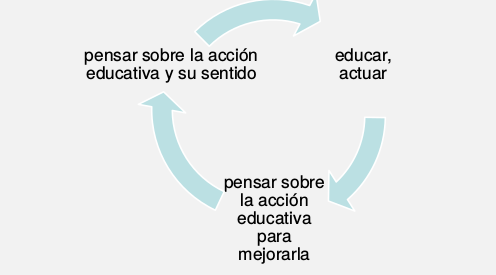
\includegraphics[scale=0.5]{\preffix/img/Circulo.png}

\small{Fuente: Material para las clases de \profe.}
\label{Circulo}
\end{figure}

\paragraph{Educar para ayudar a crecer} A veces confundimos educación con formación. 
%
Es habitual pensar en la educación como el medio para introducirse en un mercado laboral y para ello es necesaria una formación en conocimientos bastante amplia.
%
Poco a poco se va transformando la sociedad en su conjunto hacia un concepto de educación más amplio, más integrador de las diferentes facetas humanas.

"Education is not the learning of facts, but the training of the mind to think" \footnote{En español: La educación no es el aprendizaje de hechos, sino el entrenamiento de la mente para pensar.} es una frase de Einstein.
%
Einstein no hablaba de crecer sino de aprender a pensar. 
%
Una interpretación de esta frase se basa en entender que \textit{pensar} es una acción muy amplia. 
%
De hecho, el crecimiento que se busca en la educación es un crecimiento de las potencias propias (Inteligencia y Voluntad), por lo que, tal vez, Einstein no andaba desencaminado.

Es reconfortante y alentador descubrir que la propuesta educativa dada a los futuros educadores es la que uno traía ya pensada de casa.
%
Es confirmador de la vocación ver que la idea y el sueño de uno para su acción profesional coincida con la de los expertos en la materia.


\subparagraph{Armonía de todas las dimensiones} 
%
Es tremendamente aclaradora la metáfora de la poda.
%
Para forjar el carácter de los educandos es necesario cultivar y dejar crecer, pero puede haber momentos de poda.
%
La poda de una viña, por ejemplo, no quita solamente los sarmientos muertos o los que no dan fruto, sino que también puede interesar cortar sarmientos que dan poco fruto para que vuelvan a crecer más fuertes y fructíferos.

Esta metáfora de la poda resulta interesante. 
%
¿Merecerá la pena un castigo\footnote{Entendiendo castigo desde la definición Psicológica asociada a los refuerzos.} en una situación ambigüa o mediocre para que el educando pueda crecer?



\paragraph{Manipulación} 
%
Este es un tema que se discute poco desde un punto de vista ético y moral.
%
Todas las personas buscan influir en los demás, desde decisiones poco importantes hasta decisiones vitales.
%
¿Quién no ha vivido una situación en la que alguien se estaba equivocando (o eso se pensaba) y se le ha intentado conducir y corregir? 
%
Eso podría estar claro que no es una manipulación ya que se trata por el bien del otro.
%
¿Y si, en esa corrección, el corrector sale beneficiado y busca el cambio de actitud del corregido porque también sale beneficiado?
%
Los límites de la manipulación se difuminan porque es difícil ponderar la importancia que se le está dando al bien de la otra persona y al bien propio.
%
¿Y si busco el bien de un tercero?
%
Como docente podría interesar influir en un determinado estudiante para que modificara su actitud, no tanto por su propio bien personal, sino por el bien de los demás alumnos.
%
¿Quién no ha escuchado "Tu siéntate ahí, calladito y no molestes."?
%
Se están silenciando dimensiones propias de la libertad y no se está buscando el bien para esa persona.
%
¿Es esto una manipulación? ¿Se considera simplemente influencia? ¿Es éticamente correcta?

Como conclusión es importante destacar que, cuando mostramos el fin de una determinada influencia o persuasión, estamos salvaguardándonos de caer en una manipulación.
%
Además, es importante hacer capaz a la otra persona de pensar por sí misma. 



\paragraph{Cuando no educar: Nunca}
Una tentación de la profesión docente es a reducir al ámbito escolar la labor educativa.
%
Si un profesor se encuentra con alumnos por la calle que están realizando un acto de vandalismo, la opción fácil es no educar pasando desapercibido y no interviniendo.
%
Tal vez en un acto vandálico es más fácil intervenir.
%
¿Y si están de botellón? ¿Sería necesario intervenir? 
%
Si hacemos caso a que no se debe no educar nunca, lo ideal sería intervenir.

Un ejemplo menos drástico y más fácil sería a la hora de cruzar la acera. 
%
El docente es educador también fuera del centro escolar y su ejemplo es importante.
%
¿Qué educación ofrece a los alumnos que los profesores crucen mal? 
%
¿O que fumen?
%
Es importante ser ejemplares en todo momento, no sólo en el centro o sus proximidades.




\newpage
\section{Condiciones, elementos y ámbitos para educar}

En este tema se sigue trabajando una idea: el educador no causa el crecimiento del alumno. 
%
El docente sólo pone las condiciones necesarias para que ese crecimiento se pueda dar.

Todos hemos oído y experimentado que el aprecio por parte de los profesores es importante. 
%
Esta idea se ha visto apoyada por investigaciones modernas. 
%
Para que se puedan producir aprendizajes es necesaria la activación de la amígdala cerebral y éste fenómeno se da con mayor intensidad en estados anímicos positivos: cuando el alumno se siente apreciado y aceptado.

El fenómeno de la indefensión aprendida se relaciona mucho con las condiciones de competencia percibida y confianza.

\begin{defn}[Indefensión Aprendida]
Condición de un ser humano o animal que ha aprendido a comportarse pasivamente, con la sensación subjetiva de no poder hacer nada y que no responde a pesar de que existen oportunidades reales de cambiar la situación aversiva, evitando las circunstancias desagradables o mediante la obtención de recompensas positivas.
\end{defn}

Existe la creencia de que este fenómeno se produce con gran frecuencia e intensidad en las aulas de matemáticas. 
%
Decimos creencia porque no se han encontrado investigaciones que lo constaten científicamente.

Es fundamental como profesor conocer que estas condiciones son necesarias para el aprendizaje\footnote{Entendiendo aprendizaje como crecimiento y ejercicio de las potencias racionales o entrenamiento de la mente para \textit{pensar matemáticamente}.} y más fundamentalmente todavía para profesores de matemáticas donde la autocompetencia percibida puede ser muy escasa, con la consiguiente falta de autoconfianza.

\subparagraph{Contribución:} Una condición sorprendente es la de contribuir.
%
Parece instaurado en el sentido común que a los niños y adolescentes más movidos hay que darles responsabilidades para que no se aburran.
%
Pero parece que va más allá: parece que sentirse contribuidor es importante para los alumnos.

Este planteamiento es muy interesante para aulas donde se trabaja con la metodología de aprendizaje cooperativo, ya que hay muchas contribuciones.
%
De hecho, esta condición alerta de un posible peligro. 
%
¿Qué ocurre si uno del grupo no está siendo capaz de contribuir?
%
Será necesario plantear alguna tarea en la que esa persona pueda contribuir o tal vez otorgarle alguna responsabilidad dentro del grupo que sólo ella pueda llevar a cabo.

Por otro lado, para aulas donde no se trabaje cooperativamente ni por proyectos, ¿cómo ofrecer un sentido de contribución a los estudiantes?
%
Tal vez no es una pregunta que se pueda contestar ahora, pero sí es una pregunta a tener en mente para cada ejercicio de reflexión tras la acción docente ejercida.


\paragraph{Límites:} El P. Granda decía a los padres con los que trataba: "Los límites, pocos y bien puestos".
%
Los límites son necesarios pero no hay que sobrelimitar.
%
Hay aspectos en los que es necesario ser tajante, pero hay otros donde se puede ser más laxo.


Un aspecto sorprendente es que los límites fomentan la autonomía.
%
Al establecer con claridad un entorno de seguridad (qué se puede y qué no se puede; cuándo se puede y cuándo no) se permite una amplia libertad sin coacción por el miedo dentro de esas fronteras limitadoras.

Un aspecto de sentido común es que los límites deben ser establecidos y explicados a su debido tiempo, sobretodo con anterioridad a un posible incumplimiento.
%
Este verano, en un campamento de verano, se castigó una actitud (esconder comida en las habitaciones) sin haber especificado con anterioridad que estaba totalmente fuera de los límites mantener comida en las habitaciones.
%
Este castigo provocó el enfado de los acampados, que tuvieron que acabar aceptando y acatando un límite que no se había definido, lo que provocó un cierto deterioro en las relaciones interpersonales.


\newpage
\section{La familia como agente educativo}

Para mi futura labor como docente este tema me ha aportado fundamentalmente 2 aspectos: visión global sobre el papel de la familia y pautas concretas sobre la preparación de las entrevistas.

\subsection{Papel de la familia}

Conocer que el derecho internacional (la declaración de los derechos humanos) establece que \textit{Los padres tienen el derecho preferente a elegir la educación de sus hijos conforme a sus propias convicciones filosóficas y religiosas} resulta novedoso.
%
Esta apartado de la declaración critica regímenes totalitarios en los que la educación religiosa se prohíba (como podría ser la revolución francesa o el comunismo).

Por otro lado, aunque se establezca este derecho, no tiene porqué ejercerse mediante la elección de un centro con un ideario en concreto, sino que debe ir más allá.
%
Los padres siguen siendo los principales responsables de la educación de los hijos también en los ámbitos filosófico y religioso y por tanto no deben delegar totalmente esta función en el centro educativo.
%
No corresponde a otras personas que no sean los padres educar a los hijos según sus propias convicciones.
%
No es labor del centro reeducar a los hijos según sus convicciones, sino apoyar a los padres.

Esto es aplicable tanto a docentes que creen que su labor pasa por contrarrestar las convicciones religiosas de los padres bajo el argumento de que sea el hijo quien elija, como a los docentes que creen que su labor consiste en educar a los hijos en unas convicciones morales, religiosas y filosóficas contrarias a las de los padres.

Aunque todavía no he tengo respuesta a este conflicto, me ha resultado esclarecedor conocer la normativa internacional y poder reflexionar sobre el tema, ya que es un tema, en mi opinión, bastante enquistado en la sociedad española.
%
Hay quienes están a favor de que todos los centros sean exactamente iguales, laicos, etc. y quienes creemos en la necesidad de diversidad en los idearios de los centros, pero, ante todo, dentro del marco legal de actuación.

\subsection{Preparación de las entrevistas}

Aunque muchas de las cosas explicadas ya las tenía incorporadas en mi repertorio de actuación por el sentido común (como sería preparar una entrevista y tener claros los objetivos de la misma o tener entrevistas para hablar sobre la educación del alumno, aunque no haya surgido ningún problema), han habido algunos otros aspectos que me han resultado muy útiles.

Por ejemplo, volver a pensar en la importancia de realizar una evaluación y una reflexión al final de la acción educativa.
%
Al final de toda acción educativa (como veíamos anteriormente) es fundamental realizar una labor de introspección y reflexión; y esta práctica también incluye la realización de las entrevistas.

Además, es importante tener entrevistas en los tiempos y momentos establecidos.
%
La posibilidad de cruzarse con los padres a la salida del colegio y ahí tratar algunos temas no debería ser contemplada.
%
Tal vez hay algún tema que sí se podría tratar en ese momento, pero no es la manera de tener una entrevista.
%
No permite plantear objetivos de la entrevista, ni seguir una estructura planificada...
%
Lo ideal es tener entrevistas como entrevistas y no como charlas informales en el patio del colegio.
%
Así, ante el avasallamiento de una familia en el patio, la respuesta del docente podría ser: "Este no es el lugar ni el momento para hablar esto. ¿Porqué no te vienes un día y tenemos tranquilamente una tutoría?"




\newpage
\section{Amistad}


Por la labor que realizo en mi tiempo libre en la que tengo mucho contacto con adolescentes, partes de este tema me resultan muy familiares.
%
Sobretodo la dimensión psicológica de la amistad: 
%
he vivido de cerca \textit{crisis} de grupos de amigos adolescentes y he visto la importancia que le dan y el sufrimiento que les genera.
%
También he podido participar en la educación en la amistad fomentando relaciones de calidad, en las que se prioricen aspectos importantes y no banales de la relación; fomentando que se asuma el compromiso que supone una relación, buscando los momentos buenos pero sin huir ni escapar de los malos.

Debido a la escasez de tiempo en la exposición de este tema, hay algunas dudas que me han surgido durante mi trabajo con adolescentes pero que no he sabido resolver todavía.
%
¿Cómo tratar eficazmente con un adolescente que ha tenido un problema con sus amigos y le genera un gran sufrimiento?
%
¿Cómo gestionar los conflictos que surgen entre personas que empezaron a ser amigas con 6 años, pero que al alcanzar los 16 son realmente muy distintas y no hay manera de que se lleven bien? 
%
¿Cómo ayudar a diferenciar amistad de algo más?
%
¿Cómo tratar los conflictos cunado una de las 2 partes confunde amistad con algo más, o incluso siente la amistad como algo más, y la otra no?

Por otro lado, me ha resultado muy reforzador conocer que desde el punto de vista teórico se estudian y establecen conclusiones a las que había llegado desde mi experiencia.
%
Ahora sé que algunas de las cosas que yo pensaba son extrapolables a otras situaciones con otras personas, porque desde la investigación se confirman.

Como conclusión, para mi vida personal más que para mi labor docente, me quedo con que el modelo familiar que los hijos ven es el que aplican.
%
En mi familia siempre hemos tenido un póster que decía "Los niños aprenden lo que viven" (ver figura \ref{img:ninos})
%
Este tema me ha hecho reflexionar también sobre lo siguiente:
%
los alumnos también pueden aprender de las relaciones que yo mantenga con mis amigos y que ellos vean, ya sean las relaciones entre profesores como las relaciones con mi comunidad que algunos de ellos ven de vez en cuando.
%
Creo que yo también soy un modelo de referencia para ellos (de menor peso, obviamente, que la familia) y tengo que tenerlo en cuenta.
%
Además, si acabo formando una familia será importante que las relaciones que mantenga sean ejemplares, por mi bien y el de mis hijos e hijas.


\begin{figure}[hbtp]
\centering
\caption{Póster que siempre ha estado colgado en la cocina de mi casa.}
\label{img:ninos}
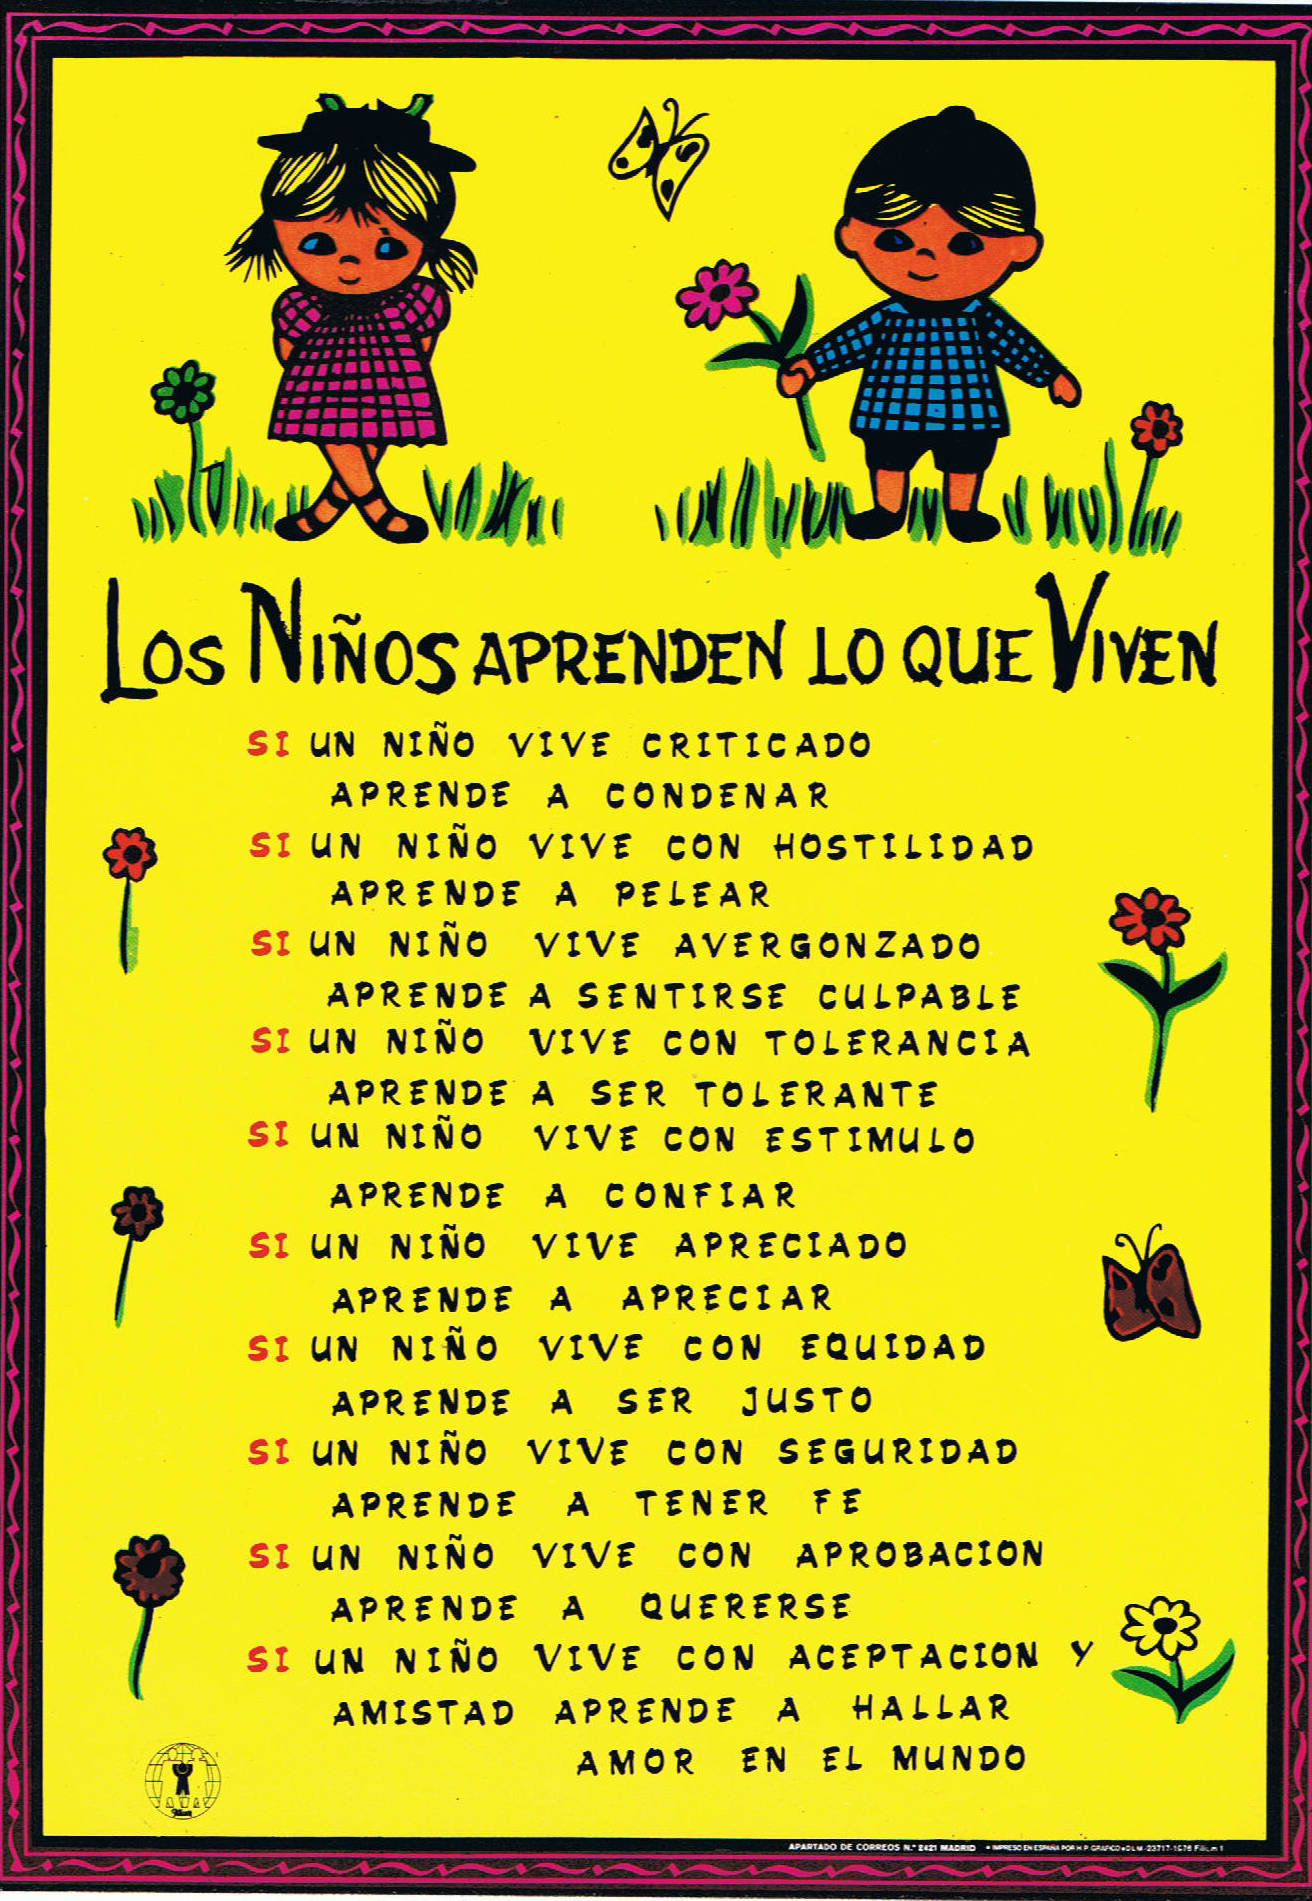
\includegraphics[scale=0.3]{\preffix/img/ninos.jpg}

\small{Fuente: \href{https://www.terapia-psicored-cam.com/psicoanalistas-articulos?lightbox=image3ht}{terapia-psicored-cam.com}}
\end{figure}





\printindex
\end{document}
